\problemname{Identifying Map Tiles}

Map websites such as Bing Maps and Google Maps often store their maps as many different image files, called tiles. The lowest zoom level (level $0$) consists of a single tile with a low-detail image of the whole map, zoom level $1$ consists of four tiles each containing a slightly more detailed version of a quarter of the map, and in general zoom level $n$ contains $4^n$ different tiles that each contain a part of the map.

One way of identifying a tile is by means of a \emph{quadkey}. A quadkey is a string of digits uniquely identifying a tile at a certain zoom level. The first digit specifies in which of the four  quadrants of the whole map the tile lies: \texttt{0} for the top-left quadrant, \texttt{1} for the top-right quadrant, \texttt{2} for the bottom-left quadrant and \texttt{3} for the bottom-right quadrant. The subsequent digits specify in which sub quadrant of the current quadrant the tile is. The quadkeys for zoom levels $1$ to $3$ are shown in Figure~\ref{fig:maps}(a).

\begin{figure}[h]
	\centering
	\subfigure[Quadkeys for zoom levels $1$ to $3$]{ \label{fig:quadkey}
\ifplastex
		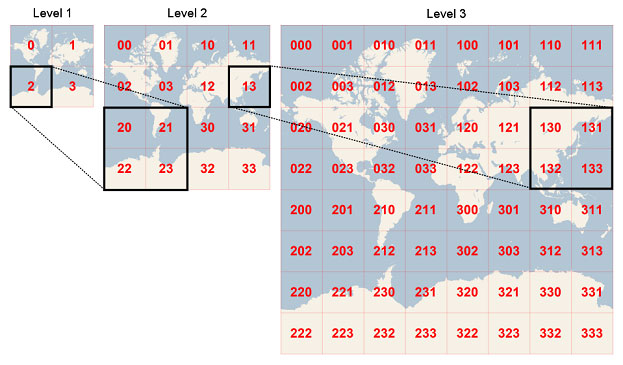
\includegraphics[width=0.85\textwidth]{maptiles.jpg}
\else
		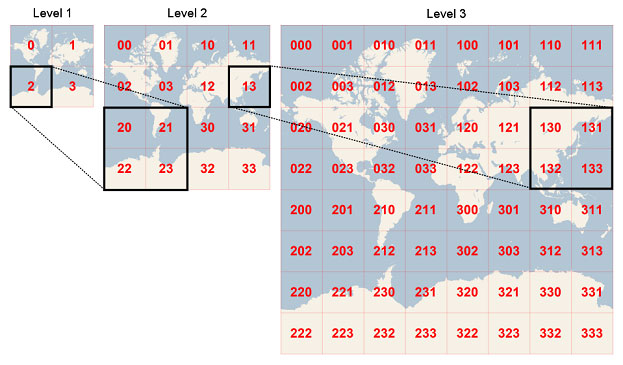
\includegraphics[width=0.6\textwidth]{maptiles.jpg}
\fi
	}
\ifplastex\else	\quad \fi
	\subfigure[Coordinates for zoom level 3]{ \label{fig:coords}
		% Ugly, use specific width to make the height equal, but problem
		% is that there's text in the left image so we can't easily use height
\ifplastex
		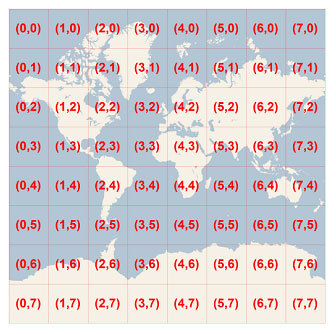
\includegraphics[width=0.90\textwidth]{maptiles2.jpg}
\else
		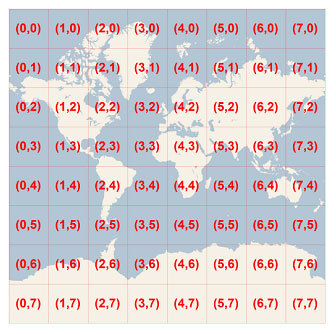
\includegraphics[width=0.338\textwidth]{maptiles2.jpg}
\fi
	}
	\caption{Visualisation of the two representations. The images are taken from the \href{https://msdn.microsoft.com/en-us/library/bb259689.aspx}{MSDN}.}
    \label{fig:maps}
\end{figure}

Another way of identifying a tile is to give the zoom level and $x$ and $y$ coordinates, where $(0,0)$ is the left-top corner. The coordinates for the tiles of zoom level 3 are shown in Figure~\ref{fig:maps}(b). Given the quadkey of a tile, output the zoom level and $x$ and $y$ coordinates of that tile.

\section*{Input}

The input consists of:
\begin{itemize}
   \item one line with a string $s$ ($1\leq \text{length}(s) \leq 30$), the quadkey of the map tile.
\end{itemize}
The string $s$ consists of only the digits `\texttt{0}', `\texttt{1}', `\texttt{2}' and `\texttt{3}'.

\section*{Output}

Output three integers, the zoom level and the $x$ and $y$ coordinates of the tile.
